






 \section{Motivation}

%\printinunitsof{in}\prntlen{\textwidth}
%\printinunitsof{in}\prntlen{\textheight}
% The text width is 6.5in -- important for plotting
% The text height is 9in

To further enhance our understanding of how fitness under drug treatment occurs, we sought to identify genomic and non-genomic basis for transcriptome differences. 
In TNBC, copy number changes have a major influence on the expression landscape \cite{wang2016integrative}.
Although many studies have analyzed CNV and differential gene expression of distinct oncogenes and tumor suppressor genes in various cancers \cite{kuzyk2015mycn, budczies2016pan, kwak2015fibroblast}, yet there has been no precise study about the relationship between CNV and differential gene expression across multiple tumor samples. It is unclear to what extent the expression level is affected by CNV at single cell level.
In Chapter 4, we established a system for identifying copy number defined clones and here we intend to exploit that to obtain scRNA-seq from the clones by mapping 10x with clonealign to CNA genotypes \cite{campbell2019clonealign}.

As \ac{DLP+} allows identification of regions of the genome that differ between the clones and the regions that are similar \cite{laks2019clonal}, therefore, we would be able to define which regions of the transcriptome might be influenced by CNA driven expression and those that might be independent of change in copy number state.

Because of the difficulty to analyse longitudinal patient samples for single cell gene expression and the lack of multiple longitudinal pre-clinical breast cancer models, these questions remain unexplored and our understanding of how they relate to triple negative breast cancer heterogeneity is limited.

Here we aimed to systematically investigate the specific relationship between copy number change and differential gene expression across timeseries TNBC PDX for which we have clonal copy number proportions already analysed in chapter 4. 

%In spite of advanced technologies and treatment, triple negative breast cancer still faces the problems of tumor recurrence and drug resistance.
%For any given difference between the types of drug resistance, for example the expression of a particular gene, it is assumed that differences arise deterministically or probabilistically in the presence of transcription factors regulating the genes in the tumors. Cancer cells in distinct cell states often exhibit important differences in functional properties depending on which genes are turned on and off resulting in sensitive or resistant phenotypes.

%The most challenging analysis is to differentiate whether the change in gene expression leading to change in cellular state is stochastic \cite{raj2008nature} or deterministic to produce the same output under similar environment.
%Previously it was shown that unique cells within a population can exhibit fluctuations in gene expression that could predict distinct phenotypes \cite{shaffer2019memory}.

%We set to explore 3 timeseries breast cancer patient derived xenografts (PDX) that were serially challenged for around 4-5 cycles with one or two drugs until and beyond they started showing resistant behaviour. The aim is to measure the magnitude of fluctuations in gene expression from sensitive to resistant phenotype.
%This study may help us better understand the correlation between CNV and differential gene expression and provide new insights into the mechanism of development and progression of cancers with potential biomarkers in triple negative breast cancer.

 \section{Synopsis}

 
 %From the previous chapter, we know that the population changes with the tumor growth from one passage to another, with and without the drugs. We see the shifts in the clones and some clones get selected and others disappear.
To explore the cellular compositions and breast cancer heterogeneity under diverse conditions, we performed scRNAseq analysis on the same 3 patient derived xenograft timeseries used as substrates in chapter 4. We acquired transcriptional signatures of 171,560 individual cells. Two libraries from CX-5461 treated samples were excluded from analysis as they did not pass our QC threshold. A total of 145,858 individual cells were taken into further transcriptome analysis, including  52,256 cells from untreated tumors, 40,754 cells from cisplatin treated tumors, 31,269 cells from cisplatin drug holiday tumors, 8,558 cells from CX-5461 treated tumors and 13,021 cells from CX-5461 drug holiday tumors (\textbf{\autoref{tab:nofcellsRNA}}).

 
%----------------------------------------------------------------

 
%To pursue our analysis at single cell RNA level, we encompassed on three main queries; (i) how to explain the data processing from our experimental design (ii) how much of the differentially expressed genes in resistant vs sensitive clones are \textit{in cis} or \textit{in trans} regulated and (iii) explore the change of expression overtime.   

To pursue our analysis at single cell RNA level, we set to explore three main questions: (i) how to best  process our experimental design data; (ii) how the gene expression changes in resistant (with drug) versus sensitive (no treatment) clones and the relationship with the copy number change (\textit{in cis} or \textit{in trans} regulated genes); (iii) how the gene expression changes over time.  

\subsection{Data processing and clonal assignments}
 From the data processing metrics, we found that batch effects in samples were largely removed by the SCTransform normalization method \cite{hafemeister2019normalization}. Differential gene expression analysis between resistant and sensitive clones was performed using \texttt{edgeR} \cite{robinson2010edger}.
Next, we used \texttt{clonealign} \cite{campbell2019clonealign} to assign RNAseq single cells to DLP+ clones and, as expected, we observed correlated clonal proportions between RNAseq clones and  DLP+ clones from chapter 4. Finally,   
we applied dimensionality reduction embeddings of the normalized gene expression levels and revealed that the clones appear to be clustering together with minor exceptions. 
%----------------------------------

%----------------------------------------------------------------

\subsection{Gene expression change over treatment states \textit{in cis} and \textit{in trans}} 
In the next section, we asked what proportion of the gene expression change in treated versus untreated samples is accounted for by the change in copy number and what proportion is independent. We defined a differentially expressed gene (DEG) to be \textit{in cis} if there was a difference in median copy number for that gene between the two compared clones, and \textit{in trans} otherwise. The global proportions of \textit{in cis} and \textit{in trans} genes in resistant versus sensitive clones were measured. Then, we looked for the magnitude of difference of upregulated or downregulated genes. Finally, we explored which pathways and individual genes are involved in resistant and sensitive clones across all timeseries PDX models. 
%We found few intersecting pathways that seems to be upregulated in all timeseries and some with 2-3

\subsection{Gene expression change over time}
Lastly, we explored the gene expression change over time in the entire gene population in each of our data sets, and we distinguished genes that were increasing or decreasing under continuous drug pressure, while observing the opposite behaviour without drug. We identified common genes that showed trends under the drug in all TNBC timeseries PDX; these could be further investigated as potential biomarkers of disease progression and tumor response.


% Please add the following required packages to your document preamble:
% \usepackage{lscape}
%\begin{landscape}
%\begin{table} 
%\centering
%\caption{Summary of \textit{in cis} and \textit{in trans} %percentages (\%) of differentially expressed genes}
%\resizebox{\textwidth}{!}{%
%\begin{tabular}{|l|p{4em}|p{4em}|p{4em}|p{4em}|p{4em}|p{4em}|}
 % \hline
%\ac{DE}-scRNAseq between clones &
 % In\_cis\_Decrease\_DownRegulated \% &
 % In\_cis\_Decrease\_UpRegulated \% &
 % In\_cis\_Increase\_DownRegulated \% &
 %In\_cis\_Increase\_UpRegulated \% &
 % In\_trans\_DownRegulated \% &
 % In\_trans\_UpRegulated \% \\
  %  \hline
%SA609-UUUU-A\_vs\_UUUU-C         & 7.9  & 4.4 & 4   & 5.2  & 40.1 & 38.4 \\
%SA609-UUUU-A\_vs\_UUUU-H         & 3.5  & 5.1 & 13  & 17.5 & 27.7 & 33.2 \\
%SA609-UTTT-A\_vs\_UUUU-C         & 14.4 & 3.3 & 1.1 & 9.3  & 32.1 & 39.8 \\
%SA609-UTTT-A\_vs\_UUUU-H         & 13   & 2.5 & 6.5 & 22.5 & 31.3 & 24.2 \\
%SA609-UTTTT-A\_vs\_UUUUU-C       & 13.2 & 3.8 & 0.9 & 10.1 & 30.5 & 41.5 \\
%SA609-UTTTT-A\_vs\_UUUUU-H       & 12.8 & 2.2 & 6.1 & 27.1 & 28.7 & 23   \\
%SA1035-UTTTT-G\_vs\_UUUUU-E      & 1.8  & 0.2 & 0.4 & 2.3  & 59.2 & 36.2 \\
%SA1035-UTTTT-H\_vs\_UUUUU-E      & 2.6  & 0.5 & 0.5 & 3.3  & 47.2 & 45.8 \\
%SA1035-UTTT-G\_vs\_UUUU-E        & 1.6  & 0.1 & 0.1 & 4.8  & 31.5 & 61.9 \\
%SA1035-UTTT-H\_vs\_UUUU-E        & 1.9  & 0.3 & 0.3 & 3.4  & 27.4 & 66.7 \\
%SA535\_UUTTTT-T\_vs\_UUUUUU-J     & 9.7  & 5.6 & 0.3 & 3.2  & 22.8 & 58.3 \\
%SA535\_UUTTT-T\_vs\_UUUUU-J       & 20.9 & 3.4 & 0.2 & 4.5  & 27.6 & 43.3 \\
%SA535\_UUTTT-S\_T\_vs\_UUUUU-J       & 20.7 & 3.4 & 0.2 & 4.4  & 28.3 & 43   \\
%SA535-UUTTT-R\_vs\_UUUUU-J       & 7.9  & 2.5 & 1.5 & 12.3 & 36.8 & 39.1 \\
%SA535\_UUTTT-T\_vs\_UUUUU-Q       & 22.5 & 4.9 & 1.5 & 20.7 & 18.4 & 32   \\
%SA535-UUTTT\_S\_T\_vs\_UUUUU-Q    & 21.7 & 5.2 & 1.4 & 21.2 & 18.1 & 32.4 \\
%SA535-UUTTT-R\_vs\_UUUUU-Q       & 16   & 4.4 & 1.8 & 31.5 & 19.9 & 26.4 \\
%SA535-UXXXX-U\_vs\_UUUUU-J       & 21.5 & 2.8 & 0.6 & 8.8  & 29.2 & 37.1 \\
%SA535-UXXXX-U\_vs\_UUUUU-Q       & 18.1 & 4.4 & 1.6 & 21.4 & 20.1 & 34.5 \\
%SA535-UXXXX-R\_vs\_UUUUU-J       & 15.3 & 2.4 & 0.6 & 7    & 40.4 & 34.3 \\
%SA535-UXXXX-R\_vs\_UUUUU-Q       & 17.1 & 3.4 & 1.9 & 27.5 & 21.8 & 28.2 \\
%SA535\_UXXXX\_M\_N\_O\_vs\_UUUUU-J & 22.1 & 4.3 & 0.4 & 6    & 28.5 & 38.7 \\
%SA535-UXXXX-M\_N\_O\_vs\_UUUUU\_Q & 19.7 & 7.7 & 1.3 & 19.3 & 18.6 & 33.5 \\
%  \hline
% \end{tabular}%
% }
%\label{tab:DEpercentageincisintrans}
%\end{table}
%\end{landscape}
%--------------------------------------------------------------

% Table generated by Excel2LaTeX from sheet 'copy number change'
% \begin{table}[htbp]
 %  \centering
 %  \caption{Percent change of copy number from one clone to another}
 %    \begin{tabular}{|l|l|l|l|}
  %     \hline
  %   Samples & \multicolumn{1}{|l}{Percent\_incis\_incr} & \multicolumn{1}{|l}{Percent\_incis\_decr} & 
  %   \multicolumn{1}{|l|}{Percent\_others} \\
  %    \hline
   %  SA609-UUUU-B\_to\_UUUU-C & 2.25 & 3.01 & 94.74 \\
 %    SA609-UUUU\_B\_to\_UUUU-H & 13.51 & 3.82 & 82.67 \\
  %   SA609-UTTT\_A\_to\_UUUU-C & 9.35 & 15.91 & 74.74 \\
  %   SA609-UTTT\_A\_to\_UUUU-H & 8.55 & 4.57 & 86.88 \\
  %   SA609-UTTTT\_A\_to\_UUUUU-C & 9.96 & 15.35 & 74.69 \\
   %  \textbf{*}SA609-UTTTT\_A\_to\_UUUUU-H & 12.27 & 5.54 & 82.19 \\
  %   SA1035-UTTTT\_G\_to\_UUUUU-E & 12.15 & 9.19 & 78.66 \\
  %   \textbf{*}SA1035-UTTTT\_H\_to\_UUUUU-E & 14.66 & 12.05 & 73.29 \\
   %  SA1035-UTTT\_G\_to\_UUUU-E & 16 & 5.63 & 78.37 \\
  %   SA1035-UTTT\_H\_to\_UUUU-E & 14.66 & 8.69 & 76.65 \\
  %   \textbf{*}SA535-UUTTTT\_T\_to\_\_UUUUUU-J & 4.5 & 19.81 & 75.69 \\
   % \textbf{*}SA535-UUTTT\_T\_to\_UUUUU-J & 3.59 & 18.63 & 77.78\\
   %  SA535-UUTTT\_S\_T\_to\_UUUUU-J & 3.51 & 18.53 & 77.96 \\
   %  SA535-UUTTT\_R\_to\_UUUUU-J & 2.03 & 1.54 & 96.43 \\
  %   SA535-UUTTT\_T\_to\_UUUUU-Q & 9.89 & 12.2 & 77.91 \\
   %  SA535-UUTTT\_S\_T\_to\_UUUUU-Q & 10.42 & 12.44 & 77.14 \\
  %   SA535-UUTTT\_R\_to\_UUUUU-Q & 7.92 & 4.85 & 87.23 \\
%\textbf{*}SA535-UXXXX\_U\_to\_UUUUU-J & 7.19 & 18.45 & 74.36 \\
   %  SA535-UXXXX\_U\_to\_UUUUU-Q & 11.84 & 11.59 & 76.57 \\
   %  SA535-UXXXX\_R\_to\_UUUUU-J & 6.8 & 15.94 & 77.26 \\
   %  SA535-UXXXX\_R\_to\_UUUUU-Q & 14.37 & 10.06 & 75.57 \\
   %  SA535-UXXXX\_M\_N\_O\_to\_UUUUU-J & 4.53 & 18.69 & 76.78 \\
   %  SA535-UXXXX\_M\_N\_O\_to\_UUUUU-Q & 9.27 & 12.36 & 78.37 \\
  % \hline 
   
% \end{tabular}%
%\label{tab:copynumberchange}%

 % \small\textbf{(* Resistant vs sensitive clones at the last time point of treatment cycle)}.
%\end{table}%

%-------------------------------------------------------------------------
% Please add the following required packages to your document preamble:
% \usepackage{lscape}

%\begin{landscape}
%\begin{table}
%\centering

 %\caption{Summary of number of differentially expressed genes \textit{in cis} and \textit{in trans} in major clones}


%\resizebox{\textwidth}{!}{%
%\begin{tabular}{|l|p{3.8em}|p{3.8em}|p{3.8em}|p{3.8em}|p{3.8em}|p{3.8em}|}
%\hline
%DE scRNAseq between clones &
 % In\_cis\_Decrease\_DownRegulated &
 % In\_cis\_Decrease\_UpRegulated &
 % In\_cis\_Increase\_DownRegulated &
 % In\_cis\_Increase\_UpRegulated &
 % In\_trans\_DownRegulated &
 % In\_trans\_UpRegulated \\
 % \hline
%SA609-UUUU-B\_vs\_UUUU-C           & 79  & 44  & 40  & 52   & 399  & 382  \\
%SA609-UUUU-B\_vs\_UUUU-H           & 127 & 186 & 471 & 636  & 1005 & 1207 \\
%SA609-UTTT-A\_vs\_UUUU-C           & 655 & 150 & 48  & 425  & 1466 & 1817 \\
%SA609-UTTT-A\_vs\_UUUU-H           & 352 & 69  & 177 & 611  & 850  & 659  \\
%SA609-UTTTT-A\_vs\_UUUUU-C         & 603 & 174 & 43  & 461  & 1394 & 1894 \\
%\textbf{*}SA609-UTTTT-A\_vs\_UUUUU-H         & 435 & 75  & 208 & 922  & 975  & 783  \\
%SA1035-UTTTT-G\_vs\_UUUUU-E        & 55  & 7   & 11  & 71   & 1841 & 1125 \\
%\textbf{*}SA1035-UTTTT-H\_vs\_UUUUU-E        & 93  & 18  & 19  & 116  & 1661 & 1612 \\
%SA1035-UTTT-G\_vs\_UUUU-E          & 35  & 3   & 2   & 106  & 696  & 1368 \\
%SA1035-UTTT-H\_vs\_UUUU-E          & 69  & 11  & 11  & 124  & 1004 & 2440 \\
%\textbf{*}SA535\_UUTTTT-T\_vs\_UUUUUU-J      & 469 & 271 & 13  & 155  & 1102 & 2814 \\
%SA535\_UUTTT-T\_vs\_UUUUU-J        & 599 & 97  & 6   & 128  & 791  & 1240 \\
%SA535\_UUTTT-S\_T\_vs\_UUUUU-J     & 595 & 97  & 5   & 126  & 811  & 1235 \\
%SA535-UUTTT-R\_vs\_UUUUU-J         & 38  & 12  & 7   & 59   & 177  & 188  \\
%SA535\_UUTTT-T\_vs\_UUUUU-Q        & 831 & 183 & 57  & 765  & 681  & 1184 \\
%SA535-UUTTT\_S\_T\_vs\_UUUUU-Q     & 834 & 200 & 54  & 812  & 696  & 1243 \\
%SA535-UUTTT-R\_vs\_UUUUU-Q         & 294 & 80  & 33  & 578  & 365  & 483  \\
%\textbf{*}SA535-UXXXX-U\_vs\_UUUUU-J & 697 & 91  & 21  & 286  & 948  & 1204 \\
%SA535-UXXXX-U\_vs\_UUUUU-Q         & 695 & 167 & 61  & 820  & 771  & 1324 \\
%SA535-UXXXX-R\_vs\_UUUUU-J         & 448 & 70  & 18  & 203  & 1178 & 1002 \\
%SA535-UXXXX-R\_vs\_UUUUU-Q         & 646 & 130 & 70  & 1038 & 823  & 1063 \\
%SA535\_UXXXX\_M\_N\_O\_vs\_UUUUU-J & 746 & 145 & 14  & 202  & 961  & 1307 \\
%SA535-UXXXX-M\_N\_O\_vs\_UUUUU\_Q  & 753 & 296 & 48  & 739  & 710  & 1281 \\
%  \hline

%\end{tabular}
%}

%\label{tab:numberofDEgenesincistrans}

%  \small\textbf{(* Resistant vs sensitive clones at the last time point of treatment cycle}.
%\end{table}
%\end{landscape}

%----------------------------------------------------------------------























\begin{table}[htbp]
  \centering
   \caption{Number of genes in DE* of resistant versus sensitive clones and their regulation status in all TNBC PDX series}
     \begin{tabular}{|l|l|l|}
     \hline
     \multicolumn{1}{|l|}{\textbf{No. of genes**}} & \multicolumn{1}{|l|}{\textbf{Percent genes (\%)}} & \textbf{Gene regulation} \\
     \hline
     \multicolumn{1}{|l|}{\textbf{SA609-TNBC}} &   &  \\
     438 & 12.9 & In\_cis\_Decrease\_DownRegulated \\
     76 & 2.2 & In\_cis\_Decrease\_UpRegulated \\
     214 & 6.3 & In\_cis\_Increase\_DownRegulated \\
     926 & 27.3 & In\_cis\_Increase\_UpRegulated \\
     966 & 28.4 & In\_trans\_DownRegulated \\
     778 & 22.9 & In\_trans\_UpRegulated \\
     \multicolumn{1}{|l|}{\textbf{SA1035-TNBC}} &   &  \\
     93 & 2.6 & In\_cis\_Decrease\_DownRegulated \\
     18 & 0.5 & In\_cis\_Decrease\_UpRegulated \\
     19 & 0.5 & In\_cis\_Increase\_DownRegulated \\
     116 & 3.3 & In\_cis\_Increase\_UpRegulated \\
     1661 & 47.2 & In\_trans\_DownRegulated \\
     1612 & 45.8 & In\_trans\_UpRegulated \\
     \multicolumn{1}{|l|}{\textbf{SA535-TNBC-cisplatin}} &   &  \\
     473 & 9.8 & In\_cis\_Decrease\_DownRegulated \\
     271 & 5.6 & In\_cis\_Decrease\_UpRegulated \\
     43 & 0.9 & In\_cis\_Increase\_DownRegulated \\
     253 & 5.2 & In\_cis\_Increase\_UpRegulated \\
     1068 & 22.1 & In\_trans\_DownRegulated \\
     2716 & 56.3 & In\_trans\_UpRegulated \\
     \multicolumn{1}{|l|}{\textbf{SA535-TNBC-CX-5461}} &   &  \\
     697 & 21.5 & In\_cis\_Decrease\_DownRegulated \\
     91 & 2.8 & In\_cis\_Decrease\_UpRegulated \\
     45 & 1.4 & In\_cis\_Increase\_DownRegulated \\
     345 & 10.6 & In\_cis\_Increase\_UpRegulated \\
     924 & 28.5 & In\_trans\_DownRegulated \\
     1145 & 35.3 & In\_trans\_UpRegulated \\
     \hline
     \end{tabular}%
     
   \label{tab:NumberofDEgenesandstatus}%
   
   \small\textbf{(*Differential expression, ** (FDR$<$0.01, p$<$0.05))}.
 \end{table}%















\textbf{MDK}, a growth factor, is recently reported as a key player in cancer progression and a promising therapeutic target \cite{filippou2020midkine}. It showed positive dynamics with continuous drug treatment. 


 % Table generated by Excel2LaTeX from sheet 'Sheet1'
\begin{table}[htbp]
   \centering
   \caption{Upregulated 4 \textit{in cis} cancer related significant genes selected from cloud plots in each of 4 PDX timeseries}
     \begin{tabular}{|r|l|l|}
     \hline
     \multicolumn{1}{|l|}{TNBC PDX ID} & Selected gene ID & Gene\_Regulation \\
     \hline
     \multicolumn{1}{|l|}{TNBC-SA609} & ID2 & in trans-upregulated \\
       & FIS1  & in cis-upregulated \\
       & CRABP1  & in cis-upregulated \\
       & TMEM147  & in cis-upregulated \\
     \multicolumn{1}{|l|}{TNBC-SA1035} & YWHAZ & in cis-upregulated  \\
       & PRKDC  & in cis-upregulated \\
       & COX6C  & in cis-upregulated \\
       & UQCRB  & in cis-upregulated \\
     \multicolumn{1}{|l|}{TNBC-535-cisplatin} & OLA1  & in cis-upregulated \\
       & CYB5A  & in cis-decrease-upregulated \\
       & KLF6   & in cis-upregulated \\
       & ELF3B  & in cis-upregulated \\
     \multicolumn{1}{|l|}{TNBC-535-CX-5461} & ID2  & in cis-decrease-upregulated \\
       & NDUFB2 & in  \\
       & MARCKS  & in trans-upregulated \\
       & BUB1  & in trans-upreg \\
       \hline
    \end{tabular}%
  \label{tab:selected4genestable}%
  \end{table}%
%-----------------------------------------------------------
























\extra {text for conclusion of chapter4}
In the TNBC-SA609 system the fitness landscape is inverted wherein
clones more fit in the untreated regime (H, D) are less fit in the treated regime, whereas less fit clones in the untreated regime (A, B) are the most fit clones under treatment. This pattern is
mirrored in two independent TNBC PDX lines treated with cisplatin, namely TNBC-SA535 and TNBC-SA1035. In TNBC-SA535, clones G, C, and B are drug-sensitive, meaning they could not survive drug pressure, while A and D are drug resistant because they are showing high fitness coefficient in the presence of drug. Also,the former have higher relative fitness in untreated versus treated regimes, while the latter exhibit an inverted fitness pattern. Similarly, in TNBC-SA1035, drug-sensitive clones consist of clones E, B, and A, while the drug-resistant group comprises clones H, I, and G. From untreated
to treated, the first group goes from high to low fitness, while the second group goes from low to high fitness. \textbf{\autoref{fig:landscapefitness}} summarises the reversal in the fitness landscape in response to cisplatin treatment in TNBC-PDX model systems.










%Next we compared the emerging clone under drug pressure with the clone that could not survive the repeated drug exposures. We identified the following significantly up regulated pathways:
%- Apoptosis, Epithelial mesenchymal transition, Hypoxia, mitotic spindle, MTORC1 signaling, MYC targets-V1, P53 pathway, TGF Beta signaling, TNFA signalling via NF-$\kappa$B, UV response up, UV response down, KRAS signaling, Angiogenesis, PI3K AKT MTOR signaling, unfolded protein response.

\begin{figure}
\centering
\includegraphics[width=\textwidth]{Figures/SA609Rxnew.pdf}
	
\caption[SA609 TNBC PDX clonal dynamics with and without treatment.]
	{\small
	\textbf{SA609 TNBC PDX clonal dynamics with and without treatment.}
	    \textbf{(a)} Heatmap representation of copy number profiles of 841 cells, grouped in 6 phylogenetic clades 
	    \textbf{(b)} Phylogeny (simplified type II sitka tree) of cells over the SA609-Un-Rx where nodes are groups of cells (scaled in size by number) with shared copy number genotype and edges represent distinct genomic copy number change points (sitka markers). \textbf{(c)} Observed clonal abundances \textbf{(d)} distribution over magnitude of difference between selective coefficients of pairs of clones \textbf{(e, f, g, h)} Analogous plots for the treated branch (n=1,593 cells).
	}
	\label{fig:SA609Rxnew}
\end{figure}


\begin{figure}
\centering
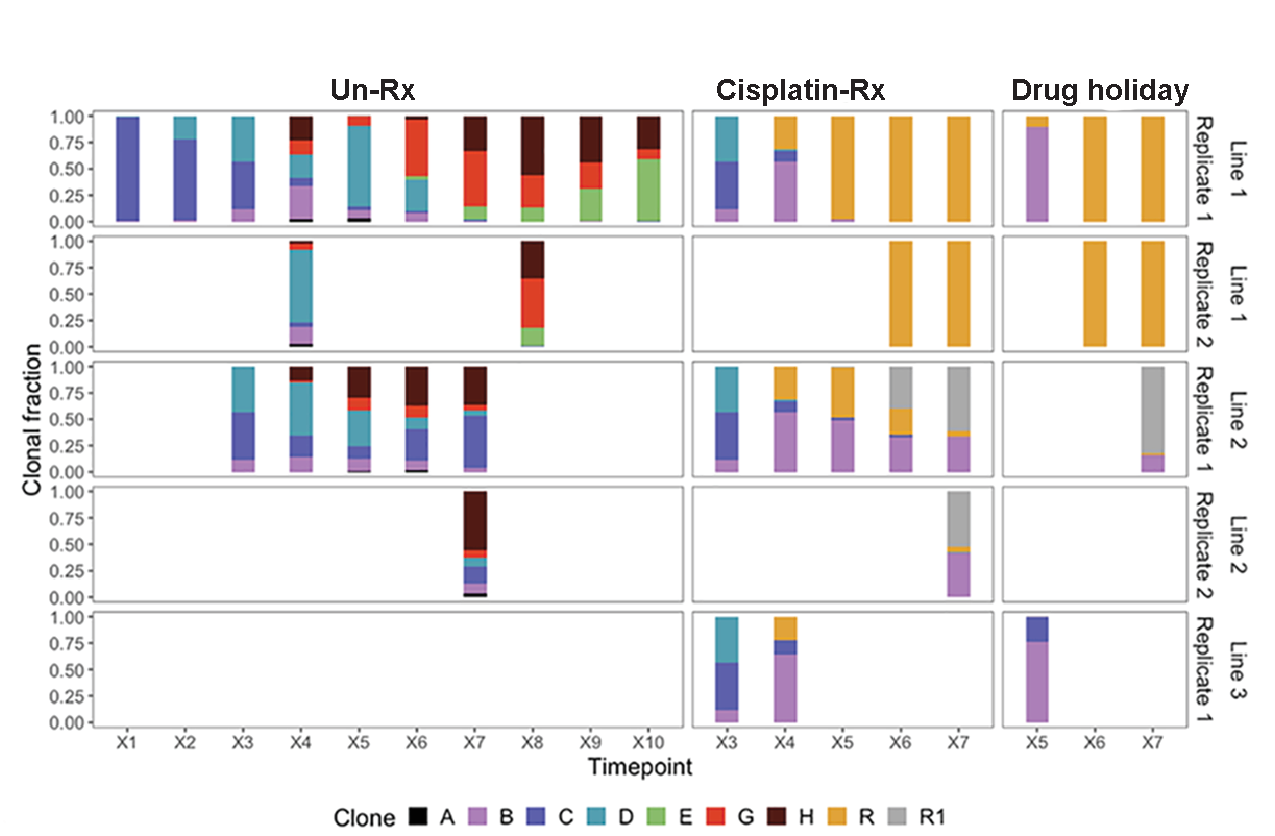
\includegraphics[width=\textwidth]{Figures/SA609barplotanalysis.pdf}
	
\caption[TNBC-SA609 PDX reproducible clonal dynamics with and without treatment]
	{\small
	\textbf{TNBC-SA609 PDX reproducible clonal dynamics with and without treatment.}
	    In both Line 1 and Line 2, the derivatives of clone B (R and R1) sweep the population. Line 3 confirms the same dynamics of clonal proportion with reversal of fitness at X5 in drug holiday sample where clone R is not fit in the absence of drug.
	}
	\label{fig:SA609barplotanalysis}
\end{figure}

%%%%%%%%%%%%%%%%%%%%%%%
\begin{figure}
\centering
\includegraphics[width=\textwidth]{Figures/SA1035Rxnew.png}
	
\caption[SA1035 TNBC PDX timeseries clonal dynamics under drug perturbation]
	{\small
	\textbf{SA1035 TNBC PDX timeseries clonal dynamics under drug perturbation.}
	    \textbf{(a)} Heatmap representation of copy number profiles of
2,015 cells, grouped in 11 phylogenetic clades  \textbf{(b)}Phylogeny (simplified type II sitka tree) of cells over the SA1035-Un-Rx where nodes are groups of cells (scaled in size by number) with shared copy number genotype and edges represent distinct genomic copy number change points (sitka markers). \textbf{(c)} Observed clonal abundances \textbf{(d)} distribution over magnitude of difference between selective coefficients of pairs of clones \textbf{(e, f, g, h)} Analogous plots for the treated branch (n=1,596 cells).
	}
	\label{fig:SA1035Rxnew}
\end{figure}
%%%%%%%%%%%%%%%%%%%%%%

\begin{figure}
\centering
\includegraphics[width=\textwidth]{Figures/SA535analysis.png}
	
\caption[SA535 TNBC PDX timeseries clonal dynamics under drug perturbations]
	{\small
	\textbf{SA535 TNBC PDX timeseries clonal dynamics under drug perturbations.}
	     \textbf{(a)} Heatmap representation of copy number profiles of
2,015 cells, grouped in 11 phylogenetic clades  \textbf{(b)} Phylogeny (simplified type II sitka tree) of cells over the SA535-Un-Rx where nodes are groups of cells (scaled in size by number) with shared copy number genotype and edges represent distinct genomic copy number change points (sitka markers). \textbf{(c)} Observed clonal abundances \textbf{(d)} distribution over magnitude of difference between selective coefficients of pairs of clones \textbf{(e, f, g, h)} Analogous plots for the treated branch (n=1,425 cells).
	}
	\label{fig:SA535analysis}
\end{figure}
%%%%%%%%%%%%%%%%%%%%%%%%%


\fitness expression old
While transcription phenotype clusters tracked with genotypic clones in the untreated series     (Fig. 6), analysis of scRNAseq from the parallel treated samples indicated that phenotypes were     also impacted by cisplatin (Pearson correlation of DLP+ clones and clonealign  scRNAseq      clones  =  0.99,   Supplementary  Fig.  8A).  Global  transcription  effects  generating  increased phenotypic  volume30  (Fig.  8A)  and  transcriptional  velocity31  (Fig.  8B  and  Supplementary     Fig.  8B)  were  observed  as  a  function  of  time  on  treatment.	As  nearly  all  tumour  cells      were  clone  R  from  X5  UTT   onwards  in  the  treatment  series,  we  attributed  transcriptional     changes to phenotypic plasticity (Fig. 8C,D and Supplementary Fig. 8C,D). Globally, 27 genes     exhibited monotonic linear and coordinated activity as a function of time on treatment (Fig. 8C).     Modified pathways included previously confirmed cisplatin-resistance metabolic processes such      as oxidative phosphorylation 32, TNFA signaling via NFKB 33–35, E2F targets 36 and hypoxia 37–40     (Supplementary Table 8).  From these pathways specific gene expression trajectories (Fig. 8E)     exemplified systematic response to sustained treatment, relative to the untreated and holiday      regimes. A minor component of the phenotypic volume was reversible (Fig. 8A) on drug holiday,     indicating only modest or partial reversibility of gene expression of clone R (Fig. 8E, X5-X6, X6-X7, Rx and Rx-H) for some genes (CEBP, NDUF7, MYC).
%------------------------------------------------
In high fitness clones (resistant) with high level amplifications as distinguishing features, we noted accompanying \textit{in cis} clone-specific differential gene expression in CRABP1 in resistant clone of SA609 TNBC PDX (clone R with XY copies of Chr15q) and  TCF4 in resistant clone of SA609 (clone R with XY copies of Chr20q) and of TNBC
CRABP1 on chr15p, TCF4 on chr 18q --------

%--------------------------------------------------
\Overall {Narrative of chapter 4:}
You know which cross reference to put in that's pretty important I think the narrative is this couple things I just wanted to go over so the first thing is in the untreated setting we have these four PG axes two of which show strong evidence of at least a couple of clones really exhibiting patterns of positive select so I think that much is clear there are two model does not show that right and then the 535 also potentially doesn't really show that I think the free model is shifted to the right and then relative to but what I'm talking about of course is figure 5A right so so this is this is important because I think what we're trying to say is that in the untreated regime there is still like positive selection happening it's not just drift and I think the end result of that that that I think makes that compelling **** thing so one is we've course do the mixture experiments in 609 to validate this and the 2nd is that switches with treatment so it really does suggest that when you change the put it select the pressure on and then in the fitness values changed in Mr rectories change that then then that is also evidenced that that their selection operating so so I think we just have to be a little delicate with how we make these points though because the evidence evidence isn't super strong from you know from the expectation that and the distribution over the expectation that you know there's there's 11 cone has positive selection over the other that's that's the main thing I wanted to talk about making any sense are you guys look like you have confused looks like faces I'm looking at the figures five and six side by side we have the basically the comparison and thinking needed so I said six or nine is the one that doesn't seem actually seems like it has a have the opposite. 4.55min.


{Single cell RNAseq global proportion of resistant vs sensitive clones presented high \textit{in trans}-regulated gene expression variations than \textit{in cis}-regulated genes.}

\subsubsection{Gene co-expression network analysis apprise biological processes relationship}

- Contrasting Frequencies and Effects of cis- and trans-Regulatory Mutations Affecting Gene Expression (read this paper)
%----------------------------------------------------------
   Clonal competition and fitness costs of platinum resistance. Having established quantification of CNA associated subclone fitness, we next asked how clone-specific fitness is influenced under drug treatment. We tested how cisplatin, a standard therapy for primary TNBC,  impacted the stability of the fitness landscape of the three independent PDX TNBC series (SA609, SA535, SA1035). For each series, wWe generated a separate branch of the TNBC timeseries passages model where we administered cisplatin (2mg/kg,  Q3Dx8 i.p. max) serially over at least four successive passages to induce drug resistance (Fig 1b, Supplementary      Fig.  5B,C,  Supplementary  Information).	Gradual onset of platinum resistance was confirmed physically in each series with progressive reduction in tumour growth inhibition (Supplementary Fig X).  For  each  serially  treated  tumour,   a  parallel   set      of  transplanted  mice  were  left  untreated,  establishing  corresponding  drug  ‘holiday’ samples     (Fig. 1bA). We coded the treated passages with ‘T’ and untreated with ‘U’, initialised by the first untreatedX3     untreated (U) passage.  In each series, we observed an inversion of the CNA clone fitness landscape (Fig 6b, left and right panels), resulting in suppression of clones that dominated under no treatment and/or the emergence of previously unobserved CNA genotypes. Thus in SA609, The first treatment passage (X4 UT) exhibited rapid tumour shrinkage      (>50%  of initial size).	However X5 UTT, X6 UTTT  and X7 UTTTT  had progressively less      response,  indicating  drug  resistance  and  positive  growth  kinetics  (Supplementary  Fig. 5E).     dDecomposing the growth dynamics over (X3 U; X4 UT; X5 UTT; X6 UTTT; X7 UTTTT) into clonal trajectories with DLP+ analysis revealed thatsuggested sustained cisplatin treatment inverted the fitness     landscapea.  Aa  new Clone R, derived from Clone A in the phylogeny, but with a distinct clonal     genotype (fewer copies of MYC and deletions at RB1, PRDM9 and NUDT15 loci (Fig. 67A,B)),     swept to fixation comprising 48% (X4 UT), 98% (X5 UTT), 100% (X6 UTTT) and 100% (X7     UTTTT) of cells across the treated series (Fig. 67Cb, Supplementary Fig. 3).  Notably, the high     fitness clones E, H, G, D from the untreated series exhibited low fitness coefficients in the treatment     series and were no longer detected (Fig. 6b,c7D, Supplementary Fig. 7), evident in the relative fitness ranking (Figure 6d clone bipartite fitness rank) and absolute fitness values (Fig 6d, probability of positive selection). Conversely, Clones A, B,     and C, comprising a low fitness phylogenetic superclade, distinct from high fitness clones E and     F in the untreated series, were the precursors to the resistant clone R (Fig. 7E). In the SA535 and SA1035 treatment series, the fitness inversion included observations of low to very low prevalence of clones ( 0.X to 0.Y) surviving platinum treatment (clone A, SA535; clones G,H, SA1035), with fitter clones under no treatment (SA535 clones G,A,B,C; SA1035 clones A-E). Thus, cisplatin perturbation resulted in a near complete inversion of the fitness landscape.
We also noticed that in the case of SA609, the inverted fitness is reversible (Fig. 1A, X5 UTU; X6 UTTU; X7 UTTTU) when in competition with precursor clones under no treatment
%-------------------------------------------------------------

Sample ID	Protein Change	Annotation	Functional Impact
SA1035	C242F	OncoKB: Likely Oncogenic, level NA;CIViC: NA;MyCancerGenome: not present;CancerHotspot: yes;3DHotspot: yes	MutationAssessor: impact: medium, score: 3.325;SIFT: impact: deleterious, score: 0;Polyphen-2: impact: probably\_damaging, score: 1
SA609	R213*	OncoKB: Likely Oncogenic, level NA;CIViC: Predisposing: 1;MyCancerGenome: not present;CancerHotspot: no;3DHotspot: no	MutationAssessor: NA;SIFT: NA;Polyphen-2: NA
SA532	A159P	OncoKB: Likely Oncogenic, level NA;CIViC: NA;MyCancerGenome: not present;CancerHotspot: yes;3DHotspot: no	MutationAssessor: impact: medium, score: 3.095;SIFT: impact: deleterious, score: 0;Polyphen-2: impact: probably\_damaging, score: 0.995
SA535	V147Gfs*2	OncoKB: Likely Oncogenic, level NA;CIViC: NA;MyCancerGenome: not present;CancerHotspot: no;3DHotspot: no	MutationAssessor: NA;SIFT: NA;Polyphen-2: NA


SA535: frameshift chr17:7578490) SNPEFF protein level
%-------------------------------------------------------------

*ASPH \cite{li2018expression, hou2018recent, kanwal2020aspartate, lin2019asph}
CDKN2A \cite{shahidsales2018genetic}-also tumor suppressor??
*RAB10 \cite{wang2017rab10}RAB10 overexpression promotes tumor growth and indicates poor prognosis of hepatocellular carcinoma
Recently, Rab10 has been demonstrated to be aberrantly expressed in some types of cancers and show biological significance in cancer progression \cite{he2002identification, jiang2016mir}
*UBE3C \cite{xiong2019mir, pan2015ubiquitin, zhang2020ube3c}
*YY1 \cite{wan2012yin, chinnappan2009transcription, meliala2020biological} 
YY1 is generally overexpressed in breast cancer cells and tissues.
YY1 was uniformly highly over-expressed in a wide range of human cancer cell lines and in human colon cancer tissue samples.
PFDN-   Prefoldin 1 promotes EMT and lung cancer progression by suppressing cyclin A expression
Overexpression of Canonical Prefoldin Associates with the Risk of Mortality and Metastasis in Non-Small Cell Lung Cancer. 
%-------------------------------------------------------------

- we determine whether under neutral conditions when there is no drug pressure what proportion of the transcriptomes might be copy number driven just due to the natural evolution of the copy number clones. This allows us to understand the stability of the gene expression in our timeseries models in the absence of drugs. 
 Next, we explored that if a drug being introduced into the system, how much of the drug induced change in expression is dependent on the copy number and which are independent.
%-------------------------------------------------------------
SA1035- from regression and gene network analysis:

*UQCRB-
Mitochondrial UQCRB as a new molecular prognostic biomarker of human colorectal cancer \cite{kim2017mitochondrial}

*MDK-Midkine (MDK) growth factor: a key player in cancer progression and a promising therapeutic target

SA535-cisplatin:

*BCAP31- BCAP31 drives TNBC development by modulating ligand-independent EGFR trafficking and spontaneous EGFR phosphorylation
-BCAP31, a cancer/testis antigen-like protein, can act as a probe for non-small-cell lung cancer metastasis
- BCAP31, a cancer/testis antigen-like protein, can act as a probe for non-small-cell lung cancer metastasis

*TPT1-LncRNA TPT1‐AS1 promotes tumorigenesis and metastasis in epithelial ovarian cancer by inducing TPT1 expression

*OLA1-Obg-like ATPase 1 (OLA1) overexpression predicts poor prognosis and promotes tumor progression by regulating P21/CDK2 in hepatocellular carcinoma

- Assessment of the role of translationally controlled tumor protein 1 (TPT1/TCTP) in breast cancer susceptibility and ATM signaling

*METTL5-Roles of METTL3 in cancer: mechanisms and therapeutic targeting
- Ribosome 18S m(6)A Methyltransferase METTL5 Promotes Translation Initiation and Breast Cancer Cell Growth.

*PABPC1-PABPC1 exerts carcinogenesis in gastric carcinoma by targeting miR-34c
-Expression and prognostic roles of PABPC1 in esophageal cancer: correlation with tumor progression and postoperative survival

*MARCKS-Overexpression of MARCKS indicates a poor prognosis of oral squamous cell carcinoma
-Stromal Expression of MARCKS Protein in Ovarian
Carcinomas Has Unfavorable Prognostic Value
-reported increased levels of phospho-MARCKS in clinical specimens of patients with lung cancer
-A novel predictor of cancer malignancy: up-regulation of myristoylated alanine-rich C kinase substrate phosphorylation in lung cancer

*RAC3 -Rac3 induces a molecular pathway triggering breast cancer \cite{gest2013rac3}.
 The Rho GTPases form 8 subfamilies; one subfamily comprises Rac1, Rac2, Rac3 and RhoG; the second subfamily contains Cdc42, TC10 (also known as RhoQ)
 It also was founded that RAC3 overexpression is required to maintain telomerase activity \cite{larrosa2015rac3, chan2005roles}.




%-------------------------------------------------------------
Activation of the interferon alpha signaling pathway has been shown to contribute to apoptosis and cellular senescence but is also attributed to increased migration and drug resistance depending on the interferon-stimulated genes transcribed. The mechanisms promoting the increase in interferon alpha expression and the role interferon alpha plays in IBC remain speculative. Deciphering the role of interferon alpha signaling and microenvironment crosstalk in inflammatory breast cancer
Olivia K. Provance & Joan Lewis-Wambi 
Breast Cancer Research volume 21, Article number: 59 (2019) 
\cite{provance2019deciphering}
\cite{mojic2018dark}-interferon gamma

E2F function couples proliferation and DNA repair by coordinating the induction of genes required for DNA synthesis, such as thymidine kinase (TK1) and dihydrofolatereductase (DHFR), and DNA repair, such as BRCA1, BRCA2, and RAD51 (51).
E2F binds to and regulates the promoters of multiple genes involved in cell cycle progression (e.g., cyclin E and cyclin A) \cite{wiedemeyer2014reversing, knudsen2010targeting}.

- Checkpoint kinase inhibitor AZD7762 enhance cisplatin-induced apoptosis in osteosarcoma cells
- Cell cycle checkpoint in cancer: a therapeutically targetable double-edged sword-G2M pathway upregulated related text.






%The important features of a timeseries patient-derived xenografts  that differentiate it from cross-sectional data-collection procedures \cite{kaplan1995time}:
 
 %\textbf{(a)} Repeated measurements of a given behavior are taken across time at equally spaced intervals.Taking multiple measurements is essential for understanding any given behavior is forced to evolve over time, and doing so at equal intervals give an open opportunity to clearly investigate the dynamics of that behavior manifesting at distinct time scales.
 %\textbf{(b)} The temporal ordering of measurements is preserved. Doing so is the only way to fully examine the dynamics governing a particular process. If we expect that a specific event will influence the dynamics of clones in a particular way, utilizing summary statistics will completely ignore the temporal ordering of the data and likely occlude one’s view of important behavioral dynamics.

%the relative contribution of these processes when  studied  in  tandem  is  poorly  understood  and  requires  integrated  genome-transcriptome investigation.   Moreover,  how  changes  in  genomic  architecture  brought  about  by  copy  number alterations drive etiologic processes remains understudied. Perturbations to induce fitness changes include genetic editing with cancer gene mutations, and pharmacologic drug selection to profile kinetics of therapeutic response.

While transcription phenotype clusters tracked with genotypic clones in the untreated series (\reffig{fig:exp}), analysis of scRNAseq from the parallel treated samples indicated that phenotypes were also impacted by cisplatin (Pearson correlation of \texttt{DLP+} clones and \texttt{clonealign} scRNAseq clones = 0.99, \refsupfig{sfig:rx_10x}A). Global transcription effects generating increased phenotypic volume\cite{Azizi2018-eb} (\reffig{fig:rxexp}A) and transcriptional velocity\cite{La_Manno2018-az} (\reffig{fig:rxexp}B and \refsupfig{sfig:rx_10x}B) were observed as a function of time on treatment.  As nearly all tumour cells were clone R from \textit{X5 UTT} onwards in the treatment series, we attributed transcriptional changes to phenotypic plasticity (\reffig{fig:rxexp}C,D and \refsupfig{sfig:rx_10x}C,D). Globally,  27 genes exhibited monotonic linear and coordinated activity as a function of time on treatment (\reffig{fig:rxexp}C).
Modified pathways included previously confirmed cisplatin-resistance metabolic processes such as oxidative phosphorylation \cite{lee2017myc}, TNFA signaling via NFKB \cite{lagunas2008nuclear,ito2015down,ryan2019targeting}, E2F targets \cite{zheng2020upregulation} and hypoxia \cite{lee2012hypoxia,mcevoy2015identifying,deben2018hypoxia,li2019erk} (\refsuptab{stab:pathway}). From these pathways specific gene expression trajectories (\reffig{fig:rxexp}E) exemplified systematic response to sustained treatment, relative to the untreated and holiday regimes. A minor component of the phenotypic volume was reversible (\reffig{fig:rxexp}A) on drug holiday, indicating only modest or partial reversibility of gene expression of clone R (\reffig{fig:rxexp}E, X5-X6, X6-X7, Rx and Rx-H) for some genes (\textit{CEBP}, \textit{NDUF7}, \textit{MYC}).

Together, these data show the impact of cisplatin selective pressure on the starting tumour cell population is reversible while genomic clonal competition with precursor clones is still possible, but becomes fixed once the evolutionary bottleneck narrows and purifies the population. Once fixed, a minor component of the expression landscape remains reversible. Thus, cisplatin resistance occurred in phases - first dominated by clonal selection on mixed populations, followed by transcriptional plasticity on a fixed genotype.



Then we get percentage of incis, intrans: nb\_incis/total [cosmic,cisplatin,fitness] genes * 100,  nb\_trans/total [cosmic,cisplatin,fitness] genes * 100, and voila, we have this proportion genes plots, blah blah







In spite of advanced technologies and treatment, triple negative breast cancer still facing the problems of tumor recurrence and drug resistance.
For any given difference between the types of drug resistance, for example, the expression of a particular gene, it is assumed that differences arise deterministically or probabilistically in the configuration of transcription factors regulating the genes in the tumors. Cancer cells in distinct cell- states often exhibit important differences in functional properties depending on the which genes are turned on and off resulting in sensitive or resistant phenotype.

The most challenging analysis is to differentiate whether the change in gene expression leading to change in cellular state is stochastic\cite{raj2008nature} and random or its deterministic to produce the same output under similar environment.
Cancer cells in distinct cell- states often exhibit important differences in functional properties depending on which genes are turned on and off resulting in sensitive  or resistant phenotype.
Previously it is shown that unique cells within a population can exhibit fluctuations in expression of a group of genes, that could predict distinct phenotypes \cite{shaffer2019memory}.
Un-like genomic clones that could get selected in resistant phenotype \cite{salehi2020single}, we still are not clear whether the cell-states are acquainted for this kind of behaviour or the selected states are pre-existing in the cancer population and under continues pressure shows obvious dynamics or there is a transition from one state to another that ultimately gets selected over time. Because of difficulty to analyse longitudinal patient's samples for single cell gene expression and lack of multiple longitudinal pre-clinical breast cancer models, these questions remains unexplored.

The introduction of RNA velocity in single cells has opened up new ways of studying cellular differentiation. Time derivative of the gene expression state can be directly estimated by distinguishing unspliced and spliced mRNAs in common single-cell RNA sequencing protocols. RNA velocity is a high-dimensional vector that predicts the future state of individual cells on a timescale of hours.......
Here we set to examine three breast cancer patient derived xenografts (PDX) that were serially challenged for around 4-5 cycles with platinum compound until they started showing resistant behaviour. We wanted to understand the magnitude of fluctuations in gene expression from sensitive to resistant phenotype.


\begin{figure}
\centering
 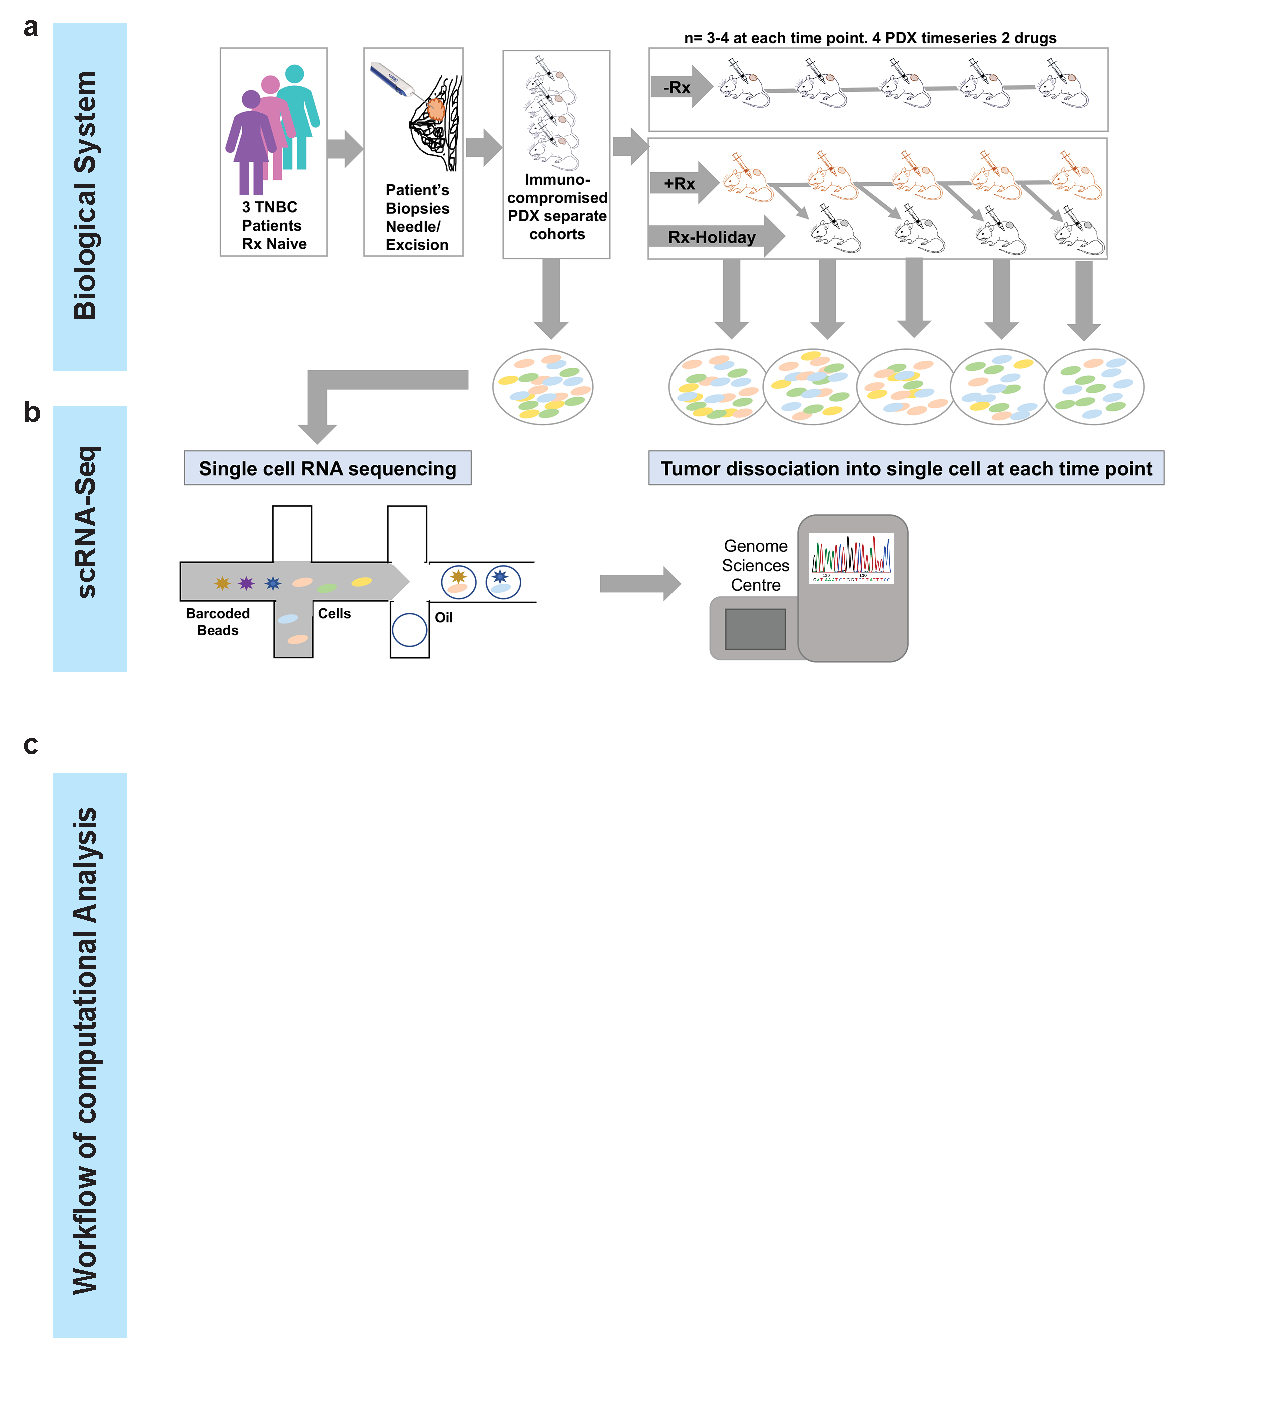
\includegraphics[width=\textwidth]{Figures/fig1schematicsoverview.pdf}
	
\caption[Schematic overview of experimental design and single cell RNA seq data analysis]
	{\small
	 \textbf{Schematic overview of experimental design and single cell RNA seq data analysis} .
	     
	}
	\label{fig:fig1schematicsoverview}
\end{figure}









Dynamics of single cell genomes and transcriptomes in response to chemotherapies

Chapter 1. To discern the stability and reproducibility of drug response properties  
1.1. To understand the range of drug response of breast cancer cell lines with respect to DNA repair deficiency- exploring NHEJ pathway in vitro for CX-5461 mechanism-(co-author paper published in Nature communication)
1.2. Large scale screening of CX-5461 in pooled cancer cell lines to discover genotype-specific vulnerabilities (on going at Broad institute)
1.3. To understand the range of drug response of breast cancer PDX in vitro
1.4. Optimization of PDX tumor processing and freezing techniques for SC whole genome, SC PBAL and SC RNA sequencing. (co-author 3 manuscripts on BioRxiv) 
1.5. Identification of tissue handling on sc-RNA seq- (co-first author manuscript in prep.)
1.6. Dissecting the maximum tolerable drug doses in NRG mice?
1.7. What are the basic patterns of drug sensitivity in PDX in vivo? (on-going)

Chapter 2. Characterizing the fitness of cancer cell in time and space

Understanding the evolutionary process within a tumor (Co-first author- “Fitness” manuscript in preparation)
1.1. Estimating the quantitative fitness of clones from time series sampling of PDX without perturbation
1.2. Do we see the same clones evolving if we physically mix early and late passages at two different dilutions?
1.3. Can we observe any change in clonal dynamics with drug perturbation? (Taxol on SA609)
1.4. What are the growth dynamics of the serially passaged PDX tumors?
1.5. Describing phenotype of all passages of PDX tumors through histological staining and expression at certain time points (SC-RNA-seq) 

Chapter 3. To understand the convergence or divergence of clonal dynamics under chemotherapeutic drugs’ selection (“lineage under drug selection” manuscript outlined)
1.1. Estimating the quantitative fitness of clones from time series sampling of PDX with drug perturbation (SA604, SA609, SA535, SA1035)
1.2.  Do the same clones mediate drug resistance or sensitivity over multiple instances of the same PDX (Using genomic markers of lineage at single cell level)
1.3. Can we compare the lineages to be compared when defined by CNA, SNV or rearrangements (Phlylogenetic tree presents same branching?) 	
1.4. To dissect the relationship between co-existing genomes and transcriptomes with chemotherapies
1.5. Can we discover new biomarkers for new targeted compounds (CX-5461) from time series sampling of PDX (CX-5461 in SA535) 

